\subsection{Zernike modes PSFs Clustering}

	\subsubsection{UMAPS}
		
		Before clustering, UMAPS for flattened PSF matrices, flattend LP coefficients matrices and PL intensities are processed. The same configuration is used for the different number of modes.
		
		\begin{table}[h!]
			\centering
			\begin{tabular}{|c|c|c|c|}
				\hline
				\textbf{Dataset type} & \textbf{Number of neighbors} & \textbf{Min distance} & \textbf{Number of components} \\
				\hline
				Zernike modes PSF & 500 & 0.5 & 1000 \\
				\hline
				LP coefficients & 500 & 0.3 & 3 \\
				\hline
				PL intensities & 500 & 0.3 & 3 \\
				
				\hline
			\end{tabular}
		\caption{UMAP parameter configurations for each of the dataset type}
		\end{table}
		
		The resulting projections are the following:
		\begin{figure*}[ht!]
			\centering
			\subfloat[2 Zernike modes LP coefficients UMAP]{%
			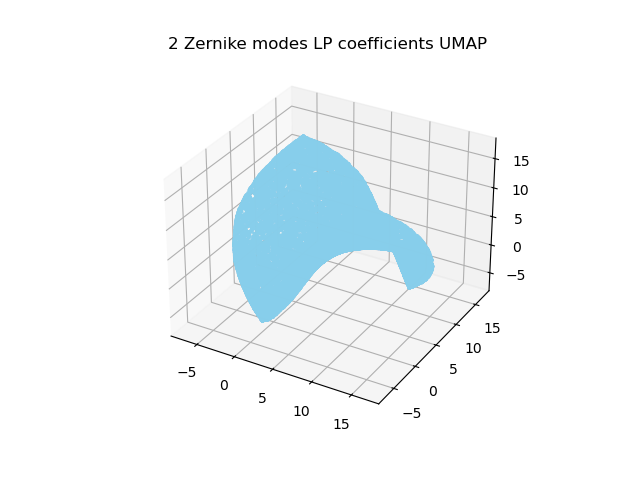
\includegraphics[ width=0.31\textwidth]{pid-2mlpcoefficientsumap.png}}
			\hspace{\fill}
			\subfloat[2 Zernike modes PL intensities UMAP]{%
			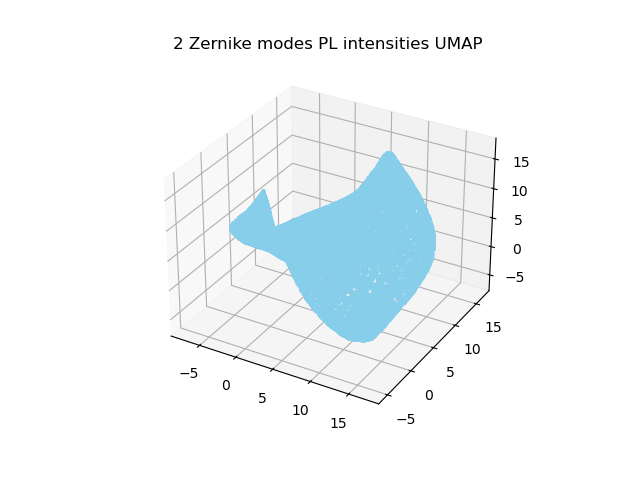
\includegraphics[ width=0.31\textwidth]{pid-2mplintensitiesumap.png}}
			\hspace{\fill}
			\\
			
			\subfloat[5 Zernike modes LP coefficients UMAP]{%
			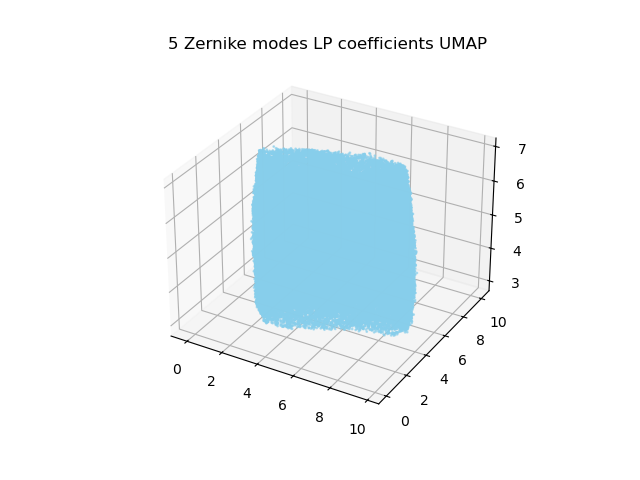
\includegraphics[ width=0.31\textwidth]{pid-5mlpcoefficientsumap.png}}
			\hspace{\fill}
			\subfloat[5 Zernike modes PL intensities UMAP]{%
			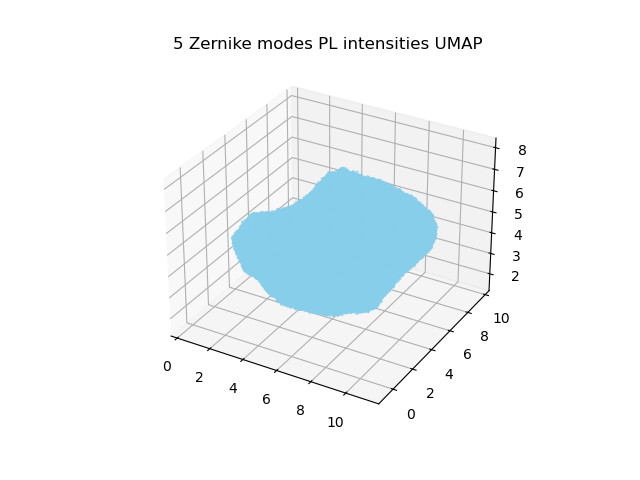
\includegraphics[ width=0.31\textwidth]{pid-5mplintensitiesumap.png}}
			\hspace{\fill}
			\\
			
			\subfloat[9 Zernike modes LP coefficients UMAP]{%
			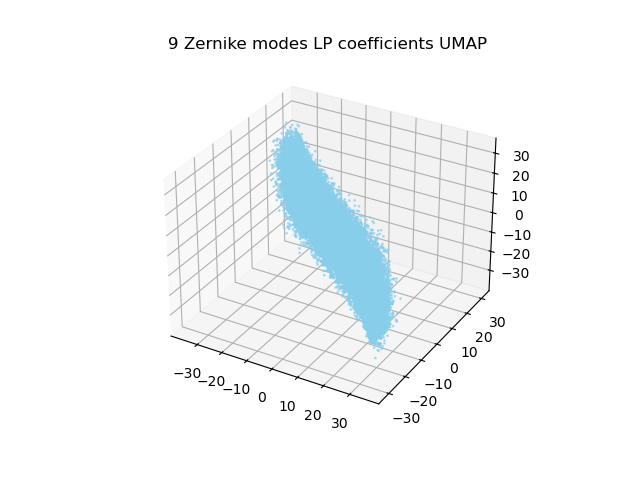
\includegraphics[ width=0.31\textwidth]{pid-9mlpcoefficientsumap.png}}
			\hspace{\fill}
			\subfloat[9 Zernike modes PL intensities UMAP]{%
			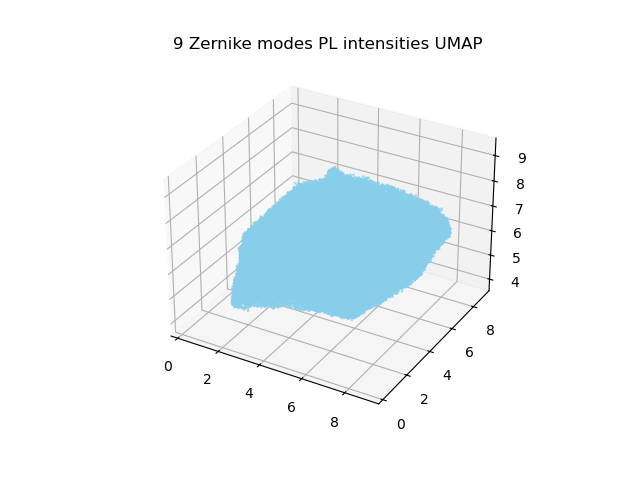
\includegraphics[ width=0.31\textwidth]{pid-9mplintensitiesumap.png}}
			\hspace{\fill}
			\\
			
			\subfloat[14 Zernike modes LP coefficients UMAP]{%
			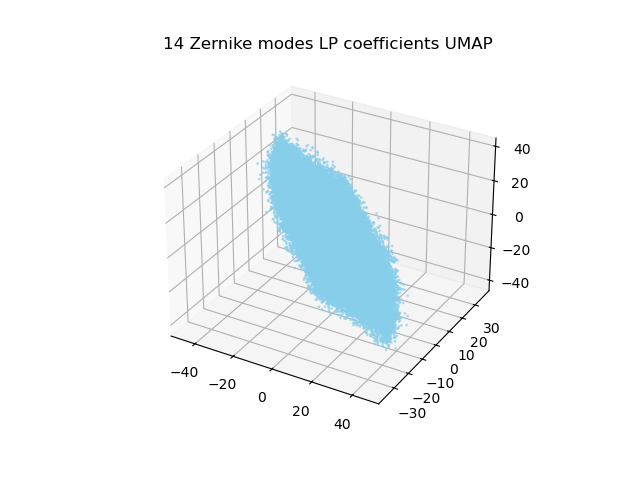
\includegraphics[ width=0.31\textwidth]{pid-14mlpcoefficientsumap.png}}
			\hspace{\fill}
			\subfloat[14 Zernike modes PL intensities UMAP]{%
			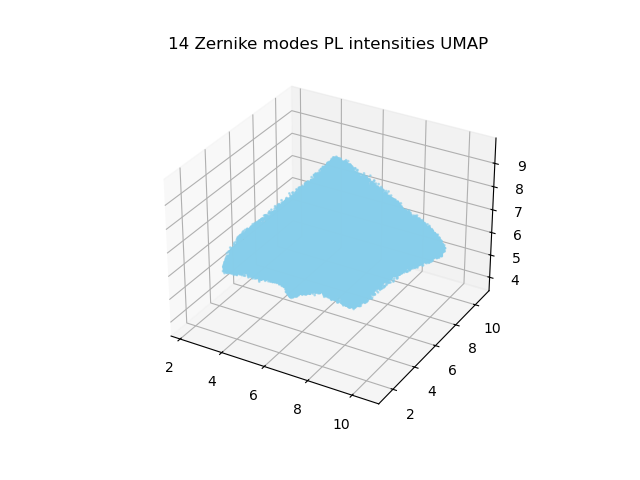
\includegraphics[ width=0.31\textwidth]{pid-14mplintensitiesumap.png}}
			\hspace{\fill}
			\\
			
			\subfloat[20 Zernike modes LP coefficients UMAP]{%
			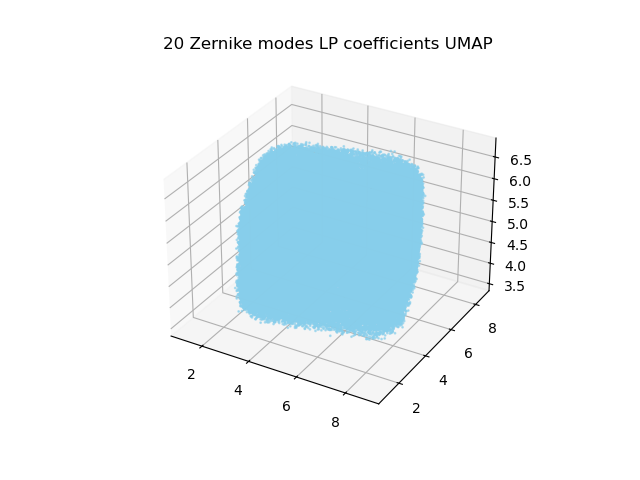
\includegraphics[ width=0.31\textwidth]{pid-20mlpcoefficientsumap.png}}
			\hspace{\fill}
			\subfloat[20 Zernike modes PL intensities UMAP]{%
			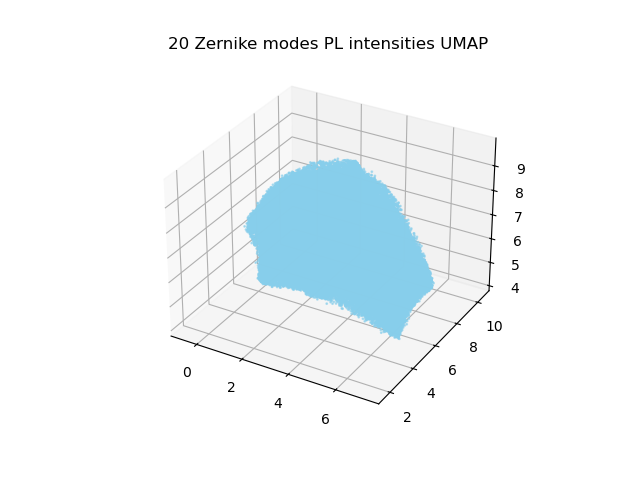
\includegraphics[ width=0.31\textwidth]{pid-20mplintensitiesumap.png}}
			\hspace{\fill}
			\\
			
			\caption{Datasets UMAPs}
		\end{figure*}
		\FloatBarrier
		
	
	\subsubsection{Clustering}
		
		Using DBSCAN I create clusters for the UMAP representations.
		
		\paragraph{2 Zernike modes}:
		\begin{table}[h!]
			\centering
			\begin{tabular}{|c|c|c|c|c|}
				\hline
				\textbf{} & \textbf{LP coeffs} & \textbf{PL intensities} & \textbf{PSF} & \textbf{Pred PSF}\\
				\hline
				\textbf{DBSCAN $\epsilon$} & 0.12 & 0.116 & 0.157 & 0.157\\
				\hline
				\textbf{DBSCAN neighbors} & 5 & 4 & 5 & 5\\
				\hline
				\textbf{Number of clusters} & 1515 & 1547 & 1466 & 1569\\
				\hline
				\textbf{Cluster density mean} & 41.89 & 42.04 & 43.57 & 40.43\\
				\hline
				\textbf{Cluster density variance} & 125.13 & 150.99 & 138.00 & 109.82\\
				\hline
				\textbf{Non noise points} & 63470 & 65046 & 63877 & 63443\\
				\hline
			\end{tabular}
		\caption{Clustering for 2 Zernike modes datasets}
		\end{table}
		\FloatBarrier
		
		\paragraph{5 Zernike modes}:
		\begin{table}[h!]
			\centering
			\begin{tabular}{|c|c|c|c|c|}
				\hline
				\textbf{} & \textbf{LP coeffs} & \textbf{PL intensities} & \textbf{PSF} & \textbf{Pred PSF}\\
				\hline
				\textbf{DBSCAN $\epsilon$} & 0.133 & 0.133 & 0.31 & 0.31\\
				\hline
				\textbf{DBSCAN neighbors} & 5 & 5 & 4 & 4\\
				\hline
				\textbf{Number of clusters} & 1528 & 1621 & 1557 & 1548\\
				\hline
				\textbf{Cluster density mean} & 35.33 & 31.70 & 29.65 & 29.93\\
				\hline
				\textbf{Cluster density variance} & 907.70 & 362.28 & 864.12 & 864.49\\
				\hline
				\textbf{Non noise points} & 53995 & 51391 & 46175 & 46333\\
				\hline
			\end{tabular}
		\caption{Clustering for 5 Zernike modes datasets}
		\end{table}
		\FloatBarrier
		
		\paragraph{9 Zernike modes}:
		\begin{table}[h!]
			\centering
			\begin{tabular}{|c|c|c|c|c|}
				\hline
				\textbf{} & \textbf{LP coeffs} & \textbf{PL intensities} & \textbf{PSF} & \textbf{Pred PSF}\\
				\hline
				\textbf{DBSCAN $\epsilon$} & 0.11 & 0.12 & 0.265 & 0.265\\
				\hline
				\textbf{DBSCAN neighbors} & 5 & 6 & 4 & 4\\
				\hline
				\textbf{Number of clusters} & 1554 & 1569 & 1408 & 1381\\
				\hline
				\textbf{Cluster density mean} & 33.87 & 34.31 & 33.06 & 33.81\\
				\hline
				\textbf{Cluster density variance} & 899.54 & 839.96 & 985.96 & 998.79\\
				\hline
				\textbf{Non noise points} & 52645 & 53847 & 46556 & 46692\\
				\hline
			\end{tabular}
		\caption{Clustering for 9 Zernike modes datasets}
		\end{table}
		\FloatBarrier
		
		\paragraph{14 Zernike modes}:
		\begin{table}[h!]
			\centering
			\begin{tabular}{|c|c|c|c|c|}
				\hline
				\textbf{} & \textbf{LP coeffs} & \textbf{PL intensities} & \textbf{PSF} & \textbf{Pred PSF}\\
				\hline
				\textbf{DBSCAN $\epsilon$} & 0.11 & 0.111 & 0.25 & 0.25\\
				\hline
				\textbf{DBSCAN neighbors} & 5 & 6 & 4 & 4\\
				\hline
				\textbf{Number of clusters} & 1492 & 1587 & 1678 & 1654\\
				\hline
				\textbf{Cluster density mean} & 37.58 & 25.88 & 26.19 & 26.68\\
				\hline
				\textbf{Cluster density variance} & 937.10 & 282.39 & 792.29 & \\
				\hline
				\textbf{Non noise points} & 56076 & 41081 & 43947 & 802.27\\
				\hline
			\end{tabular}
		\caption{Clustering for 14 Zernike modes datasets}
		\end{table}
		\FloatBarrier
		
		\paragraph{20 Zernike modes}:
		\begin{table}[h!]
			\centering
			\begin{tabular}{|c|c|c|c|c|}
				\hline
				\textbf{} & \textbf{LP coeffs} & \textbf{PL intensities} & \textbf{PSF} & \textbf{Pred PSF}\\
				\hline
				\textbf{DBSCAN $\epsilon$} & 0.109 & 0.113 & 0.25 & 0.25\\
				\hline
				\textbf{DBSCAN neighbors} & 6 & 5 & 4 & 4\\
				\hline
				\textbf{Number of clusters} & 1364 & 1524 & 1586 & 1688\\
				\hline
				\textbf{Cluster density mean} & 36.79 & 35.80 & 28.33 & 25.94\\
				\hline
				\textbf{Cluster density variance} & 870.92 & 965.84 & 861.31 & 787.24\\
				\hline
				\textbf{Non noise points} & 50189 & 54563 & 44940 & 43791\\
				\hline
			\end{tabular}
		\caption{Clustering for 20 Zernike modes datasets}
		\end{table}
		\FloatBarrier
		
		
	\subsubsection{Normalised Mutual Information}
		
		After running an NMI on the clusters these are the results:
		\begin{lstlisting}
	NMI from datasets created with 2 Zernike Modes
    		- LP coeffs and PL intensities:
    			0.8164576430824315
    		- LP coeffs and PSF: 
    			0.8175003226815989
    		- PL intensities and PSF:
    			0.7994322323774545
    		- LP coeffs and predicted PSF: 
    			0.8175646434293075
    		- PL intensities and predicted PSF: 
    			0.7983573747301721
    		- Predicted PSF and original PSF: 
    			0.8095814407687527
    				
	NMI from datasets created with 5 Zernike Modes
    		- LP coeffs and PL intensities: 
    			0.2546247849754754
    		- LP coeffs and PSF clusters: 
    			0.2761463896986409
    		- PL intensities and PSF clusters:
    			0.2169490063500632
    		- LP coeffs and predicted PSF clusters: 
    			0.28175438653504503
    		- PL intensities and predicted PSF clusters: 
    			0.21635800151194817
    		- Predicted PSF and original PSF clusters: 
    			0.5464235488639057

	NMI from datasets created with 9 Zernike Modes
    		- LP coeffs and PL intensities: 
    			0.19594140953604774
    		- LP coeffs and PSF clusters: 
    			0.19331293998931096
    		- PL intensities and PSF clusters: 
    			0.14033346512809078
    		- LP coeffs and predicted PSF clusters: 
    			0.18823201153015062
    		- PL intensities and predicted PSF clusters: 
    			0.13583799714028102
    		- Predicted PSF and original PSF clusters: 
    			0.4208027610913512

	NMI from datasets created with 14 Zernike Modes
		- LP coeffs and PL intensities: 
			0.2061877271415178
		- LP coeffs and PSF clusters: 
			0.22489998453619262
   		- PL intensities and PSF clusters: 
   			0.15638010188248286
   		- LP coeffs and predicted PSF clusters: 
    			0.22450523757936153
    		- PL intensities and predicted PSF clusters: 
    			0.15124830319698243
    		- Predicted PSF and original PSF clusters: 
    			0.3978566533293418

	NMI from datasets created with 20 Zernike Modes
    		- LP coeffs and PL intensities:
    			0.15590863566718433
    		- LP coeffs and PSF clusters: 
    			0.2096232888801945
    		- PL intensities and PSF clusters: 
    			0.11871048630190495
    		- LP coeffs and predicted PSF clusters: 
    			0.20997226177915623
    		- PL intensities and predicted PSF clusters: 
    			0.1269907541345761
    		- Predicted PSF and original PSF clusters: 
    			0.2983128702057625
	\end{lstlisting}
	
		\begin{itemize}
			\item There is a stronger relationship between LP coefficients and PL outputs than PSF to LP coefficients.
			\item The relationship between PSF and PL outputs is the weakest.
			
		\end{itemize}		 
		\begin{figure*}[ht!]
			\centering
			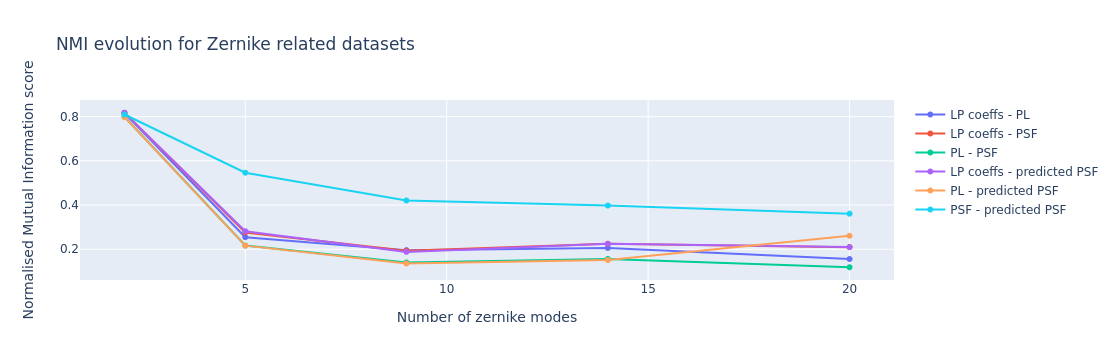
\includegraphics[width=0.7\textwidth]{pid-nmizernike.png}
			\caption{NMI evolution over Zernike related datasets}
		\end{figure*}
		
		\begin{figure*}[ht!]
			\centering
			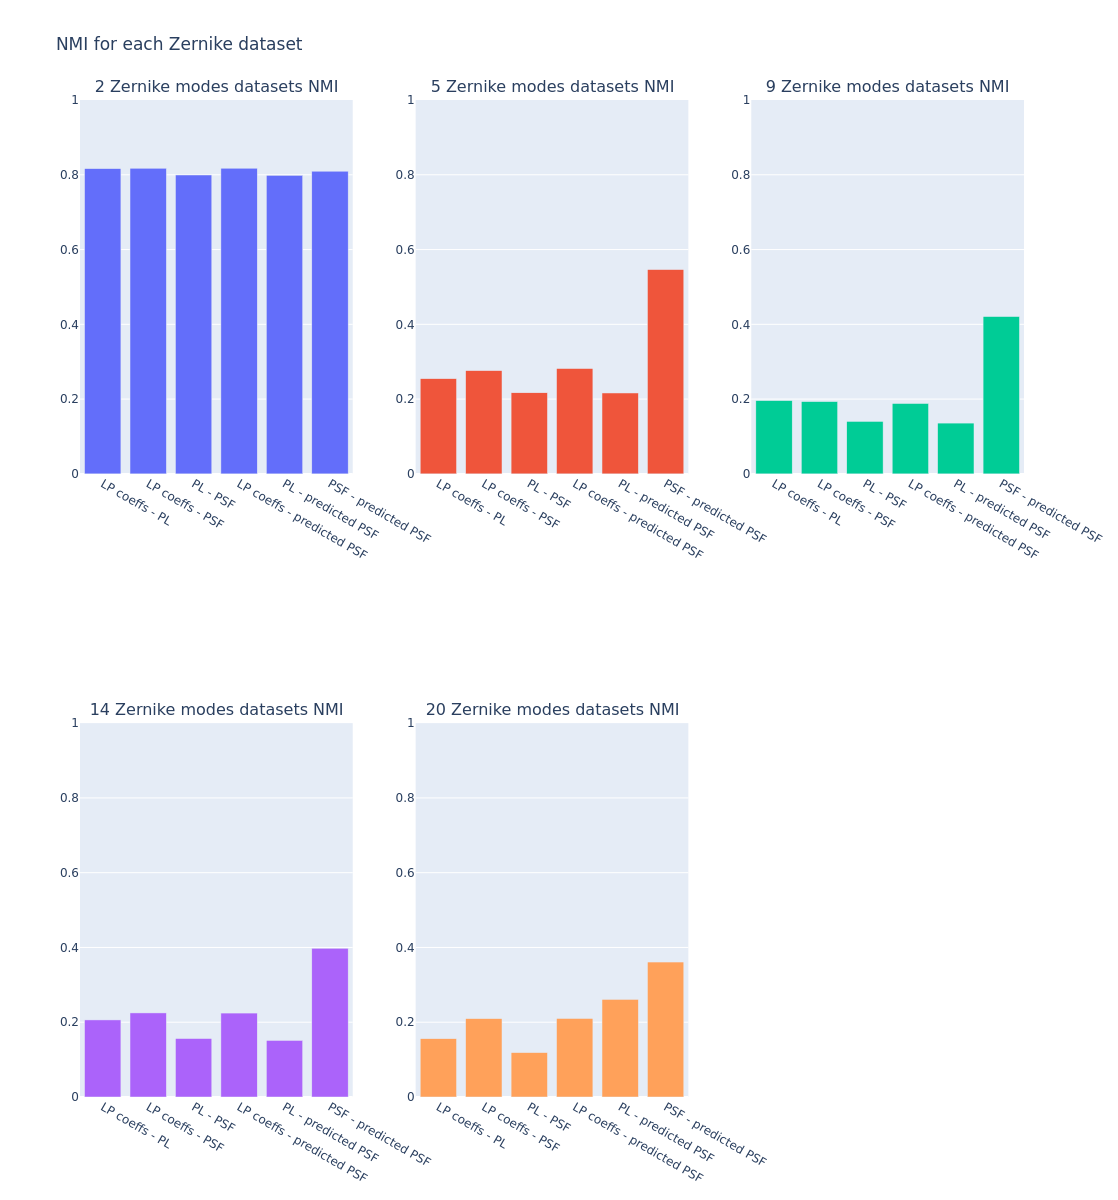
\includegraphics[width=0.7\textwidth]{pid-separatednmizernike.png}
			\caption{NMI for each of the Zernike related datasets}
		\end{figure*}